\documentclass[12pt, english]{article}
\usepackage[utf8]{inputenc}
\usepackage[T1]{fontenc}
\usepackage{graphicx}
\graphicspath{ {./images/} }
\usepackage{float}
\usepackage{babel}
\usepackage[a4paper, bindingoffset=0.2in, left=1in, right=1in, top=1in, bottom=1in]{geometry}
\usepackage{biblatex}
\addbibresource{citation.bib}
\usepackage{multicol}
\usepackage{import}


\begin{document}

\date{}
\maketitle


\thispagestyle{empty}
	
	\begin{figure}[H]
	    \vspace{-1in}
		
\includegraphics[scale = 0.5]{images/North-South-University.png}
		\centering
		\label{EscudoUABC}
	\end{figure}
	
	\begin{center}
	\vspace{0.8cm}
	\LARGE
	Post-COVID19 Psychological Distress Detection Using Machine Learning Techniques
	
	
	\vspace{1.7cm}	
	\Large
	\textbf{Junior Design Course Project (CSE299) Report}
	
	\vspace{1.3cm}
	\normalsize	
	Instructor \\
	\vspace{.3cm}
	\large
	\textbf{Dr. Shahnewaz Siddique} \\
	\text{Assistant Professor \\ Dept. of Electrical and Computer Engineering \\ North South University}

	\vspace{1.3cm}
	\normalsize	
	Submitted by \\
	\vspace{.3cm}
	\large
	\textbf{Shafayet Rajit 1921325042 \\ Mezbah Uddin Saad 1921703042}
	
	\end{center}
	
	\newpage
	
	\begin{abstract}
COVID-19 has affected people’s lives on many dimensions. Human beings could not interact with each other normally for a long time. This, along with various other issues, the pandemic had a severe impact on people’s mental health. In this project, we aim to create a machine learning model which will predict whether one is suffering from anxiety or other mental health problems based on some of the answers they provide to certain questions. This project also focuses on finding out how much COVID-19 has affected our mental health in the long run.  

There are two parts of the data collected from numerous respondents, one of that is information regarding personal lifestyle and another is a popular anxiety assessment questionnaire, GAD-7. Using this information, we have trained a machine learning model. This model will take into account the various aspects of personal lifestyle during COVID-19. After that, it will also analyze the GAD-7 score for each respondent. Finally, it will try to predict anxiety levels in individuals using only information on personal lifestyle. 

We have used the collected data to train machine learning models utilizing multiple algorithms. Among them, the decision tree algorithm has produced the highest accuracy with a score of 54.7\%. This project targets to analyze mental health using highly efficient machine learning algorithms in order to produce rapid and correct detection of psychological distress. 


	\end{abstract}

\clearpage
\tableofcontents
\clearpage
\section{Introduction}
COVID19 has affected people’s lives on many dimensions. Human beings could not interact with each other normally for a long time. This, along with various other issues, the pandemic had a severe impact on people’s mental health.

In this project, we aim to create a machine learning model which will predict whether one is suffering from depression or other mental health problems based on some of the answers they provide to certain questions. These questions will be related to their lifestyle during the COVID19 pandemic. Observing their lifestyle during the pandemic, the model will show the level of anxiety or other psychological distress one may be going through. 

This project is titled “Post-COVID19” as in our country, the number of  COVID-19 patients is gradually lessening right now. Even though there are sudden increases, the overall situation is much more bearable than before. So, we will ask the participants questions regarding their situation during COVID-19 and use that information to predict their mental health. 


\section{Problem Statement}
To build a machine learning model that will be able to detect the level of psychological distress one may experience due to their lifestyle in COVID-19.

\section{Background}
Professionals all over the world have worked to successfully detect the wellness of mental health. There was a spike in research on this field during the COVID19 pandemic as the impact became evident. Machine learning techniques have led to rapid and accurate results in these researches. After collecting the necessary data from willing participants, the researchers trained a machine learning model using suitable algorithms. Some of the popular algorithms are KNN, SVM, Logistic Regression, Random Forrest, Decision Tree, etc. 

Prout, Tracy A., et al. (2020) collected data from 2,787 people from different backgrounds and implemented random forrest algorithm to train the model. They have taken into account the demographics, history of adverse childhood experiences, current coping strategies, and current psychological distress. Their findings indicate that younger participants, women, and non-binary individuals reported higher prevalence of symptoms across all measures of distress. \cite{2}

Sau et al. (2017) manually collected data from the Medical College and Hospital of Kolkata, West Bengal on 630 elderly individuals, 520 of whom were in special care. After applying different classification methods they produced a model with the best accuracy rate of 91\% and 89\% among the two data sets of 110 and 520 people, respectively. \cite{1}

\section{Solution Process}
\subsection{Data Collection}
In order to collect data, we prepared a set of questionnaires related to lifestyle during the COVID19 pandemic. There were two parts of the questionnaire, one is about personal lifestyle and another is the GAD-7 questionnaire. 

The questions in the personal lifestyle section requested information regarding demography and lifestyle during COVID-19. The detailed questionnaire is mentioned in the appendix section. 

The second part of the questionnaire was a set of questions titled GAD-7 questions. This assessment was chosen as it has displayed good agreement between self-report and interviewer-administered assessments meaning this method can be used with confidence in both scenarios.  

The original validation study conducted on adult patients in primary care clinics in USA reported a Cronbach’s α score of 0.92 \cite{3}. Other clinical and non-clinical studies conducted in Korea, Portugal, the United States, Iran, Germany, and, Peru have similarly found excellent Cronbach’s α coefficient which shows good internal consistency of the GAD-7 scale across different populations \cite{4, 5, 6, 7, 8}. Specifically, surveys conducted on university students in Korea and college students in Portugal found Cronbach’s α coefficient to be 0.91 and 0.88 respectively, revealing excellent internal consistency [40, 41]. In Bangladesh, Faisal et al. (2021) found good internal consistency of GAD-7 (Cronbach’s α = 0.87) in a study on university students [14]. 

There are seven questions in the GAD-7 questionnaire and with each question, there is a level of severity from 0 to 3. The participant must choose the number applicable to their scenario. Then, after combining all the scores, the final score is used to determine the level of anxiety. The questions along with score levels are presented in figure 1 and figure 2.


\begin{figure}[H]
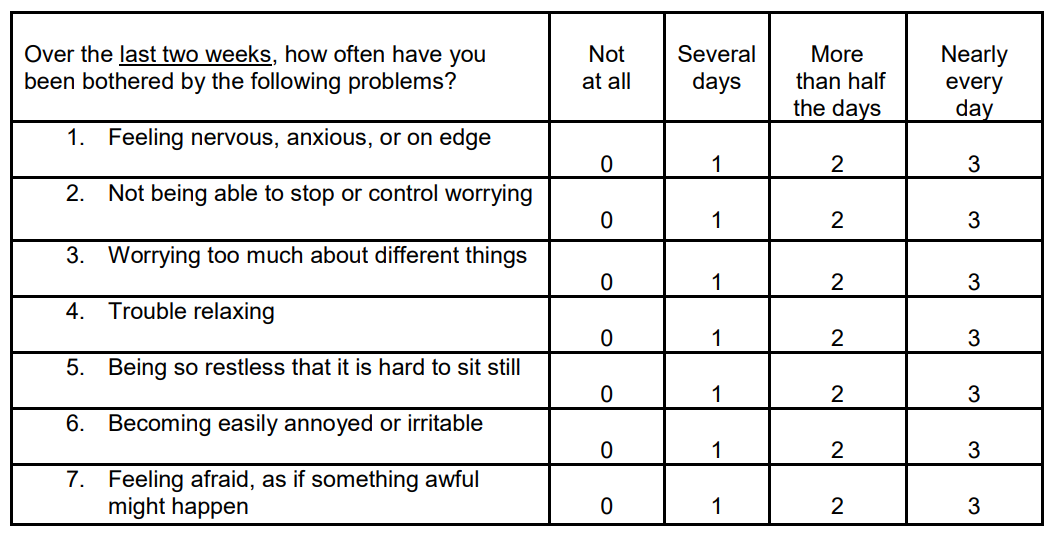
\includegraphics[width=\textwidth]{images/GAD7_questions.png}
\centering
\caption{GAD-7 Questions}
\end{figure}

\begin{figure}[H]
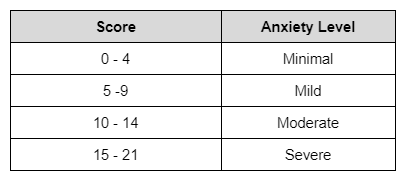
\includegraphics{GAD7_grade.png}
\centering
\caption{GAD-7 Results}
\end{figure}

We have collected the data using an online form, named Google forms, as it is easier to reach a large number of people through this medium. This data collection process was completely anonymous. Any information that may identify an individual has not been requested in this data collection process. 

\subsection{Data Processing}
We have collected 230 responses in total over the course of one month. We aimed to collect categorical data so that it is easier to process. In order to ease the management of this data, we have assigned shortened labels to each one of them. Additionally, we have simplified the categorical data by assigning indicator values to them. After collecting the data, we used visualization libraries, such as Seaborn, to analyze the data and get an overview of the dataset. 

In Figure 4, we can see that we have managed to get a balanced representation of both males and females. However, it is evident observing Figure 3 that most of the data came from people who are between the ages of 18 and 24. Similarly, if we look at Figures 5 and 6, we can draw conclusions that most of the respondents are unmarried students. Thus, in terms of demographic information, we can conclude that there is a certain amount of bias in our dataset. 



\begin{figure}[H]
    \centering
    \begin{minipage}{0.45\textwidth}
        \centering
        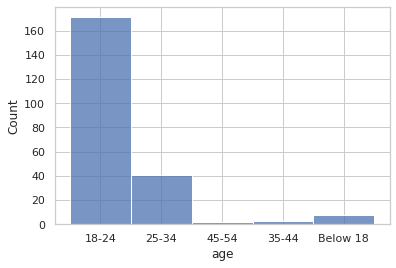
\includegraphics[width=0.9\textwidth]{images/age.png} % first figure itself
        \caption{Age}
    \end{minipage}\hfill
    \begin{minipage}{0.45\textwidth}
        \centering
        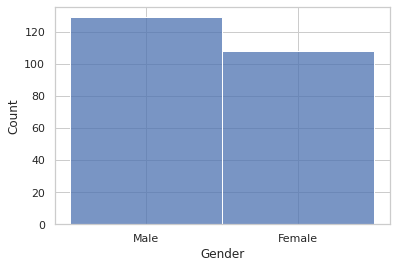
\includegraphics[width=0.9\textwidth]{images/gender.png} % second figure itself
        \caption{Gender}
    \end{minipage}
\end{figure}

\begin{figure}[h]
    \centering
    \begin{minipage}{0.45\textwidth}
        \centering
        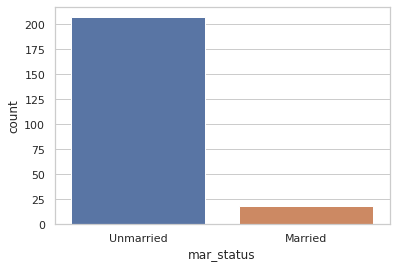
\includegraphics[width=0.9\textwidth]{images/maritial.png} % first figure itself
        \caption{Marital Status}
    \end{minipage}\hfill
    \begin{minipage}{0.45\textwidth}
        \centering
        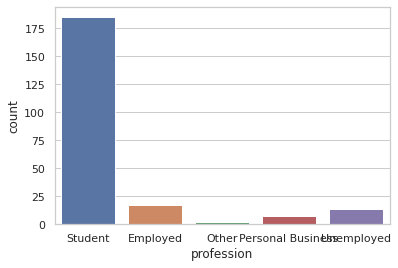
\includegraphics[width=0.9\textwidth]{images/profession.png} % second figure itself
        \caption{Profession}
    \end{minipage}
\end{figure}

Now, Figure 7 represents the family monthly income of respondents. We have assigned short terms for better visualization. The scale is stated below: 
\begin{multicols}{2}
\begin{enumerate}
  \item 'More than 1,50,00 BDT':'SRI', \item '1,20,000 - 1,49,999 BDT':'RI',
  \item '1,00,000 - 1,19,999 BDT':'HC', \item '70,000 - 99,999 BDT':'HMC',
  \item '50,000 - 69,999 BDT':'MC',  \item '30,000 - 49,999 BDT':'LMC'
  \item 'Less than 30,000 BDT':'LOI'.
\end{enumerate}
\end{multicols}

\begin{figure}[H]
    \centering
    \begin{minipage}{0.45\textwidth}
        \centering
        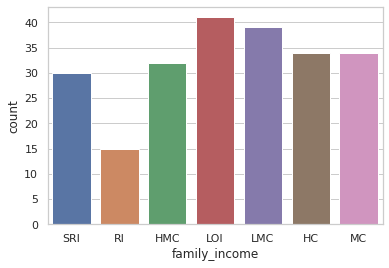
\includegraphics[width=0.9\textwidth]{images/family_income.png} % first figure itself
        \caption{Family Income}
    \end{minipage}\hfill
    \begin{minipage}{0.45\textwidth}
        \centering
        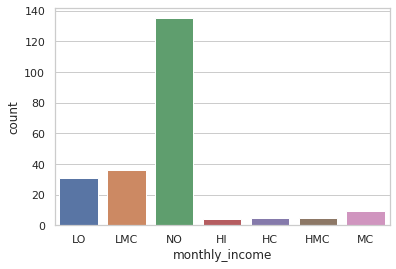
\includegraphics[width=0.9\textwidth]{images/monthly_income.png} % second figure itself
        \caption{Own Monthly Income}
    \end{minipage}
\end{figure}

In the case of Figure 8, which represents the monthly income for oneself, we have used the following scale: 
\begin{multicols}{2}
\begin{enumerate}
  \item 'More than 1,00,000 BDT':'HI', 
  \item '70,000 BDT - 99,999BDT':'HC',
  \item '50,000BDT - 69,999BDT':'HMC', 
  \item '30,000BDT - 49,999BDT':'MC'
  \item '50,000 - 69,999 BDT':'MC',  
  \item '30,000 - 49,999 BDT':'LMC'
  \item '10,000BDT - 29,999BDT':'LMC', 
  \item 'I do not have any income at the moment':'NO',
\end{enumerate}
\end{multicols}
\noindent Here, we can also see that there are respondents from various income classes in our dataset but a large number of them do not earn themselves. 

Getting infected by a disease like COVID19 definitely affects one psychologically. So, we wanted that data to predict the severity of one’s anxiety. Figure 9 represents information about whether the respondent himself/herself has contracted COVID19 and Figure 10 shows data regarding whether COVID19 has infected any of the family members. 

\begin{figure}[H]
    \centering
    \begin{minipage}{0.45\textwidth}
        \centering
        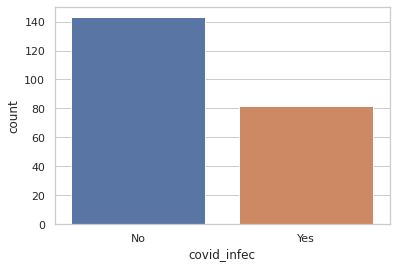
\includegraphics[width=0.9\textwidth]{images/covid_infec.png} % first figure itself
        \caption{Infected with COVID19}
    \end{minipage}\hfill
    \begin{minipage}{0.45\textwidth}
        \centering
        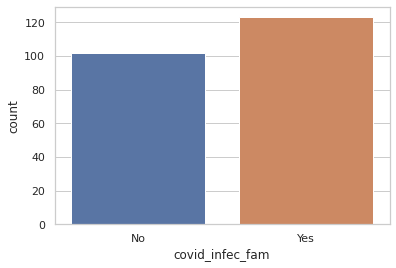
\includegraphics[width=0.9\textwidth]{images/covid_infec_fam.png} % second figure itself
        \caption{Any Family Member Infected with COVID19}
    \end{minipage}
\end{figure}

We also wanted to see how many of the respondents knowingly experienced anxiety or other psychological issues during the pandemic. Figure 11 is used to show that representation and figure 12 shows how many of them had sought professional help. It is clear that even after experiencing psychological distress, most people refuse to get mental health counseling or similar treatments. 

\begin{figure}[H]
    \centering
    \begin{minipage}{0.45\textwidth}
        \centering
        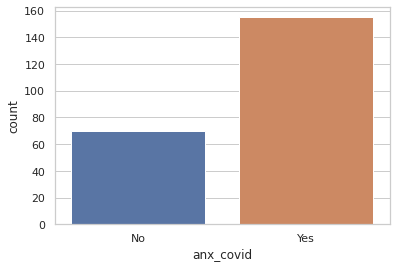
\includegraphics[width=0.9\textwidth]{images/anx_covid.png} % first figure itself
        \caption{Experienced Psychological Distress}
    \end{minipage}\hfill
    \begin{minipage}{0.45\textwidth}
        \centering
        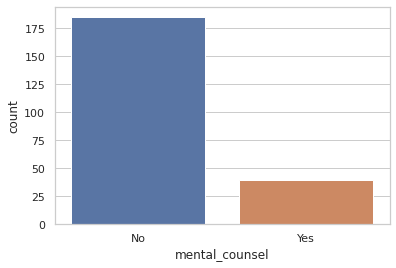
\includegraphics[width=0.9\textwidth]{images/mental_counsel.png} % second figure itself
        \caption{Received Mental Health Treatment}
    \end{minipage}
\end{figure}

There are seven questions in GAD-7 assessment and the score of each questions are summed to get the final result. We have followed the similar process to determine the level of anxiety. After adding the scores of all the questions, we have stored them in a different column. This column alone is used to understand the anxiety level of each respondent. We have also assigned labels to each final score following the GAD-7 scale(FIgure 2). To keep our dataset clean, we have dropped the individual scores of each questions as we do not need them anymore. 


\subsection{Algorithms}

There are various types of algorithms for different problems in machine learning. The problem that we are trying to solve is a classification problem meaning the model will classify whether there is a specific problem or not. In this project, we have used the following algorithms, K Nearest Neighbours, Decision Tree, and Logistic Regression. We have used statistical techniques such as SMOTE, and cross-validation. SMOTE is applied to increase the number of cases in our dataset. Cross-validation is a method to evaluate and compare learning algorithms after dividing data into multiple segments. We have also used a particular cross-validation technique, stratified K-fold sampling, to split the dataset and keep the ratio of target classes the same throughout the whole dataset. Another implemented cross-validation technique is shuffle split which randomly samples the entire dataset during each iteration to generate training and a test set. 

K-Nearest Neighbours works by observing similarities between existing data and new data. This model stores all the data and when new data is assigned, it analyzes that data by comparing it to each of the current data. When the KNN model finds data mostly similar to a particular existing data, it assigns a similar label to the new data. KNN is particularly useful for classification problems. Thus, we have implemented this model in our project.  

Decision Tree is one of the most popular models used for classification problems. It is called a tree because it works with different nodes and each of these nodes denotes an attribute. There are also branches that represent the outcome of a node. Using this tree-like feature can lead to a decision. This model has the ability to handle high-dimensional data. It is also proven to have good accuracy in classification problems. 

Logistic regression is used to predict a binary outcome based on the analysis of a dataset. It takes into account the correlation between different features of the dataset. It is one of the most commonly used algorithms in classification problems. As in this project, we are working on a classification problem, this model is suitable. 

\section{Analysis}

After applying KNN model, at first, it was able to score a test accuracy of 40\%. However, after modifying our data using SMOTE and other cross validation techniques, KNN managed to score accuracy of 53.4\%. In this model, we have used maximum 30 neighbours to train the model and it has shown the highest accuracy when 15 neighbours were considered. 

\begin{figure}[H]
    \centering
    \begin{minipage}{0.45\textwidth}
        \centering
        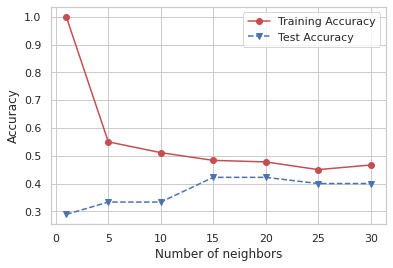
\includegraphics[width=0.9\textwidth]{images/knn_first.png} % first figure itself
        \caption{Initial KNN Accuracy}
    \end{minipage}\hfill
    \begin{minipage}{0.45\textwidth}
        \centering
        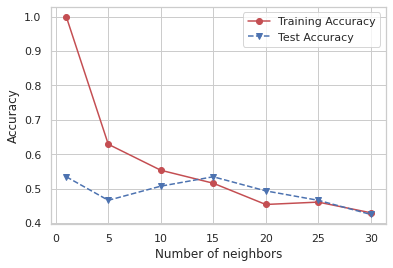
\includegraphics[width=0.9\textwidth]{images/knn_final.png} % second figure itself
        \caption{Final KNN Accuracy}
    \end{minipage}
\end{figure}

Initially, on our dataset, decision tree produced accuracy score of 35\%. After modifying our dataset, this score had risen to 54.7\%. We have used a maximum depth of 50 in this model. The algorithm has shown the highest accuracy at depth of 8.  
\begin{figure}[h]
    \centering
    \begin{minipage}{0.45\textwidth}
        \centering
        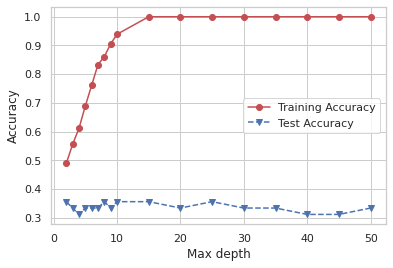
\includegraphics[width=0.9\textwidth]{images/dt_first.png} % first figure itself
        \caption{Initial Decision Tree Accuracy}
    \end{minipage}\hfill
    \begin{minipage}{0.45\textwidth}
        \centering
        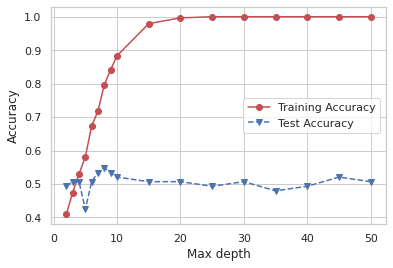
\includegraphics[width=0.9\textwidth]{images/dt_final.png} % second figure itself
        \caption{Final Decision Tree Accuracy}
    \end{minipage}
\end{figure}

Logistic regression has produced an accuracy score of 50.5\% on our dataset. Observing the confusion matrix(Figure 17), it is evident that our trained model is more accurate in predicting ‘Minimal’ and ‘Severe’ cases than other anxiety levels. 

\begin{figure}[H]
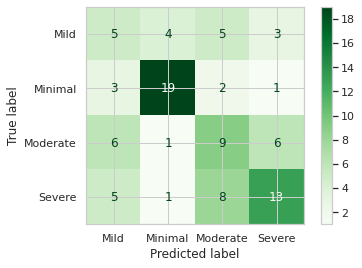
\includegraphics[scale=0.75]{images/conf_matrix.png}
\centering
\caption{Confusion Matrix}
\end{figure}

\section{Conclusion}
\subsection{Summary}
The main goal of this project was to build a machine learning model which is able to predict the general anxiety level based on their lifestyle during the pandemic. We have collected data from 230 people on their personal lifestyles and mental health. Analyzing the collected data, we have used various machine learning algorithms to build the most efficient model for this purpose. In our study, we have found that the Decision Tree has accurately predicted the outcome most of the time. The accuracy of the decision tree algorithm was 54.7\%. KNN and logistic regression managed to acquire accuracy scores of 53.4\% and 50.5\% respectively. Thus, for our dataset, decision tree has achieved higher accuracy than other algorithms.

\subsection{Limitations}
The major limitation of this project is the lack of quality data. With a larger number of data, this project would have performed better. There is also a higher number of respondents who are from a similar background and this has caused a certain level of bias in the dataset. Professionals can carry out future studies on this similar topic keeping in mind the mentioned lackings.

\section{References}
\printbibliography[heading=none] %Prints bibliography
\section{Appendix}
\appendix
\chapter{Terms}
\centering
GAD = General Anxiety Disorder
SMOTE = (Synthetic Minority Oversampling Technique)
Cronbach’s α = Cronbach's alpha is a way of assessing reliability by comparing the amount of shared variance, or covariance, among the items making up an instrument to the amount of overall variance.

\chapter{Data Collection Form}
\centering
\begin{figure}[h]
    \centering
    \begin{minipage}{0.45\textwidth}
        \centering
        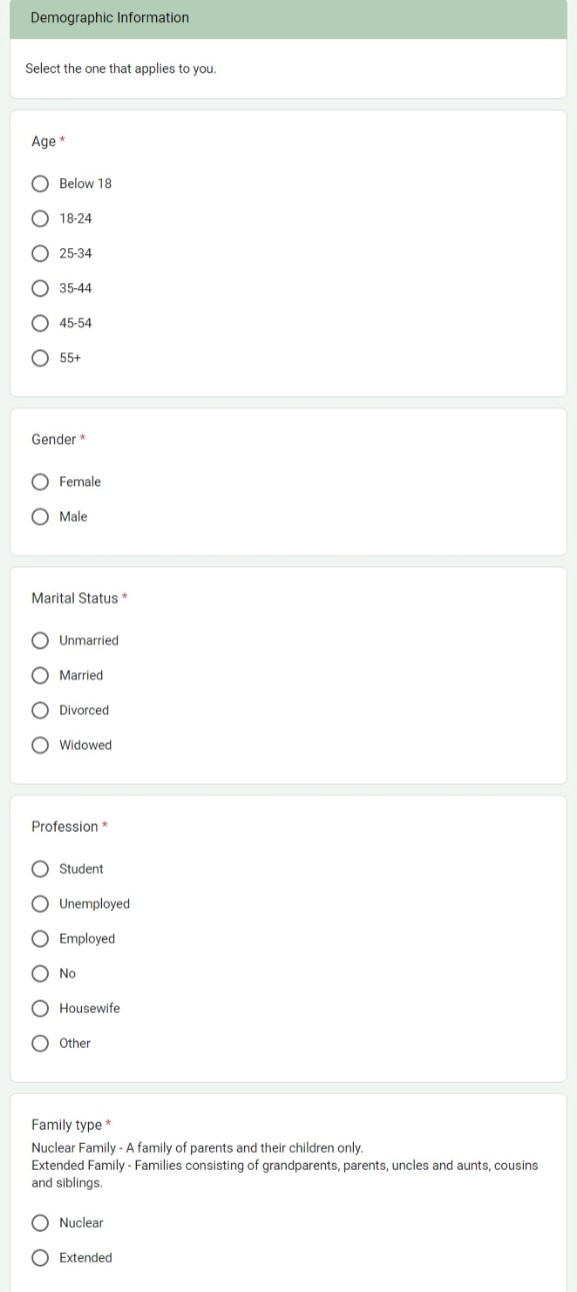
\includegraphics[width=0.9\textwidth]{images/demo.jpeg} % first figure itself
        \caption{Demographic Information}
    \end{minipage}\hfill
    \begin{minipage}{0.45\textwidth}
        \centering
        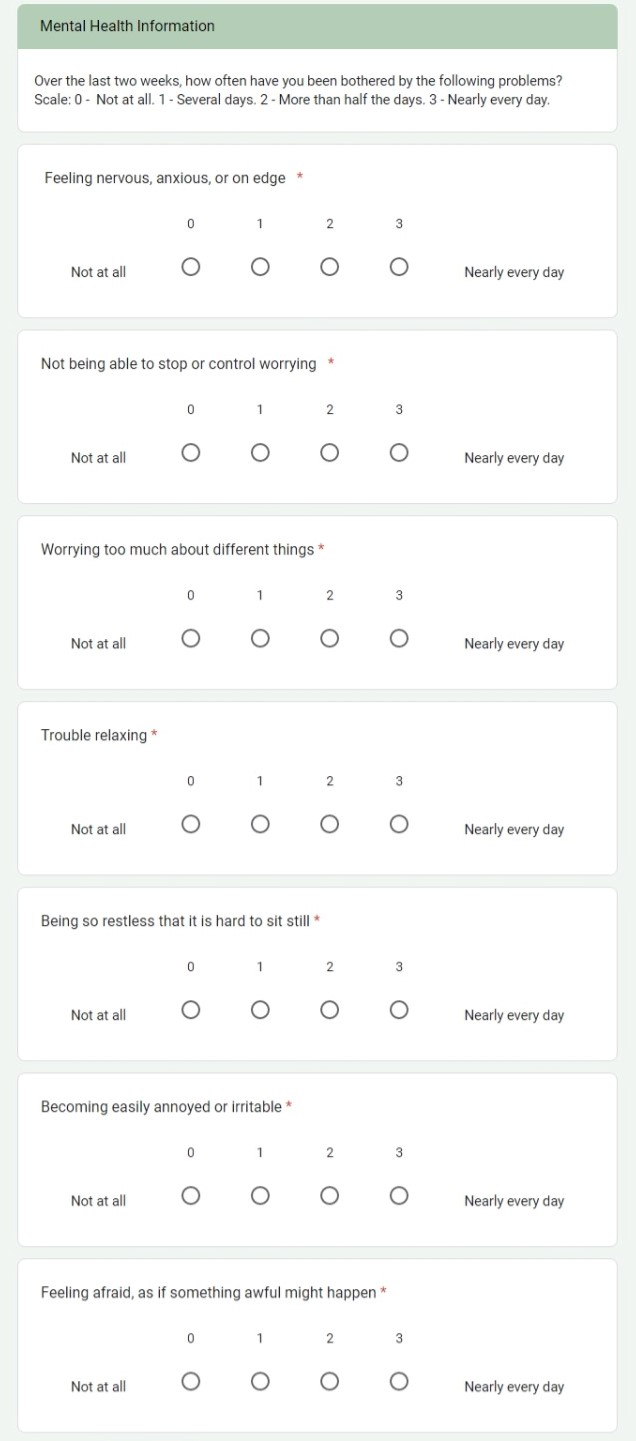
\includegraphics[width=0.9\textwidth]{images/psy.jpeg} % second figure itself
        \caption{GAD-7 Questions}
    \end{minipage}
\end{figure}

\begin{figure}[h]
    \centering
    \begin{minipage}{0.45\textwidth}
        \centering
        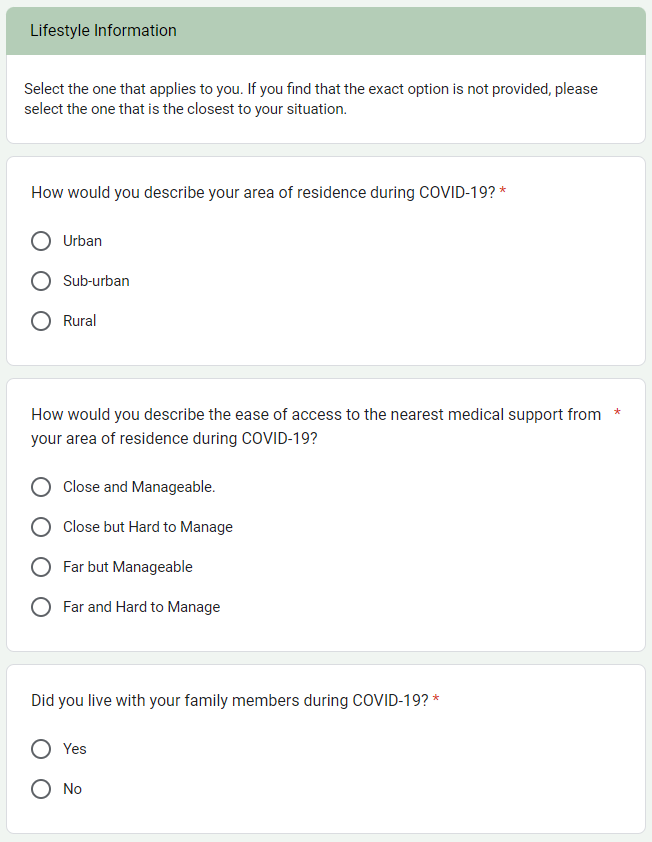
\includegraphics[width=0.9\textwidth]{images/lifestyle_1.png} % first figure itself

    \end{minipage}\hfill
    \begin{minipage}{0.45\textwidth}
        \centering
        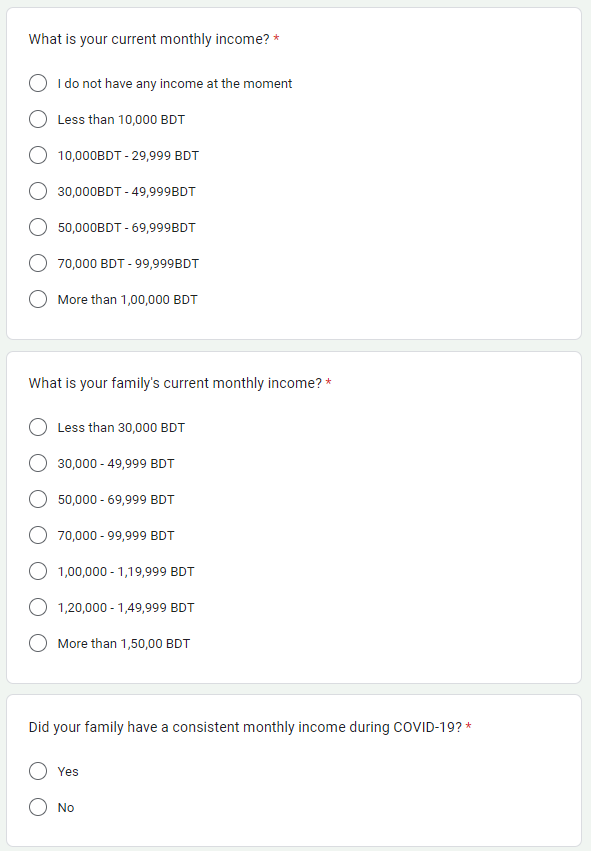
\includegraphics[width=0.9\textwidth]{images/lifestyle_2.png} % second figure itself
        
    \end{minipage}
    \caption{Lifestyle Information}
\end{figure}

\begin{figure}[h]
    \centering
    \begin{minipage}{0.45\textwidth}
        \centering
        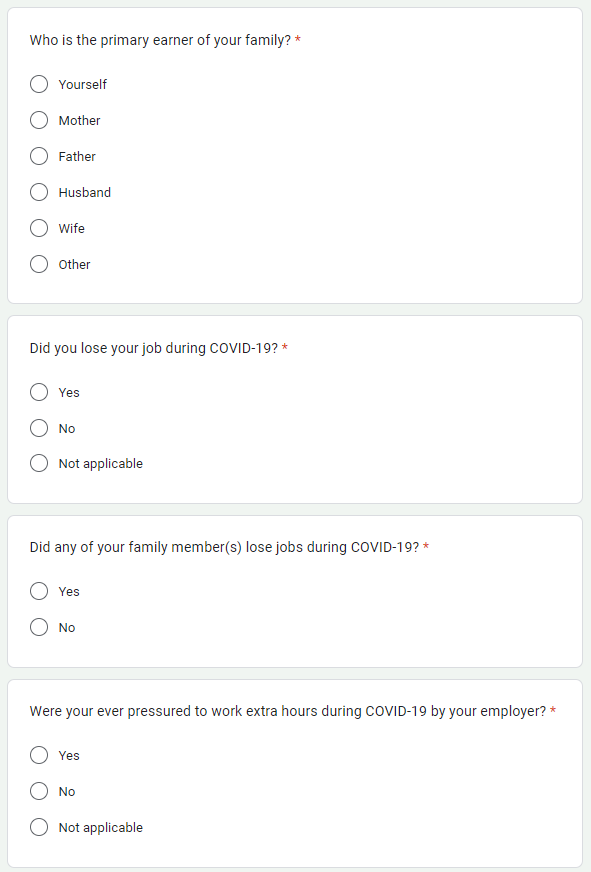
\includegraphics[width=0.9\textwidth]{images/lifestyle_3.png} % first figure itself

    \end{minipage}\hfill
    \begin{minipage}{0.45\textwidth}
        \centering
        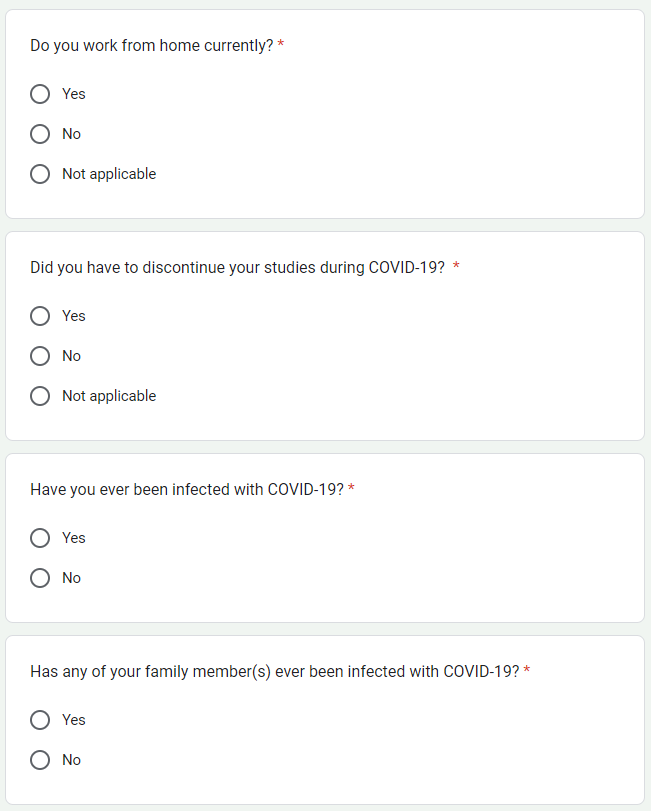
\includegraphics[width=0.9\textwidth]{images/lifestyle_4.png} % second figure itself
        
    \end{minipage}
    \caption{Lifestyle Information}
\end{figure}

\begin{figure}[h]
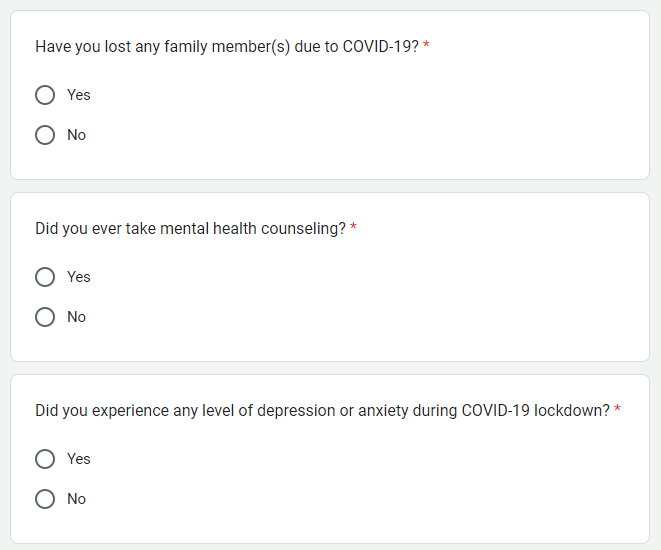
\includegraphics[scale=0.75]{images/lifestyle_5.png}
\centering
\caption{Lifestyle Information}
\end{figure}

\end{document}
